\documentclass{article}
\usepackage[utf8]{inputenc}
\usepackage[section]{placeins}
\usepackage[]{algorithm2e}

\makeatletter
\AtBeginDocument{%
  \expandafter\renewcommand\expandafter\subsection\expandafter{%
    \expandafter\@fb@secFB\subsection
  }%
}
\makeatother

\title{Optimal Code Generation for Expression Trees using Haskell}
\author{Ganesh Bhambarkar - \texttt{153050072}
\\ Sushant Shambharkar - \texttt{153050081}}
\date{November 2015}

\usepackage{natbib}
\usepackage{graphicx}
\usepackage{listings}

\usepackage{color}
 
\definecolor{codegreen}{rgb}{0,0.6,0}
\definecolor{codegray}{rgb}{0.5,0.5,0.5}
\definecolor{codepurple}{rgb}{0.58,0,0.82}
\definecolor{backcolour}{rgb}{0.95,0.95,0.92}

\lstdefinestyle{mystyle}{
    backgroundcolor=\color{backcolour},   
    commentstyle=\color{codegreen},
    keywordstyle=\color{magenta},
    numberstyle=\tiny\color{codegray},
    stringstyle=\color{codepurple},
    basicstyle=\footnotesize,
    breakatwhitespace=false,         
    breaklines=true,                 
    captionpos=b,                    
    keepspaces=true,                 
    numbers=left,                    
    numbersep=5pt,                  
    showspaces=false,                
    showstringspaces=false,
    showtabs=false,                  
    tabsize=2
}

\lstset{style=mystyle}

\begin{document}

\maketitle

\section{Introduction}  
This project involves generation of optimal code for  the machine using Aho-Johnson algorithm given an expression tree and a machine model. Bruno and Sethi show that generating optimal code is difficult, even if the target machine has only one register; specifically they show that the problem of generating optimal code for straight-line sequence of assignment statements is NP-complete.\citep{Aho:1976:OCG:321958.321970} 

On the other hand , if we restrict the class of inputs to straight line programs with no common sub-expression, optimal code generation becomes considerably easier.\citep{Aho:1976:OCG:321958.321970}  

\section{Problem Definition}
Input to the algorithm is a machine model and expression tree. Machine model contains number of registers and a set of instructions that machine supports. Expression tree is a sequence of assignment statements represented as tree.

\section{Algorithm}  
The Aho-Johnson algorithm produces machine code for a given expression tree with minimum cost. The algorithm is from dynamic programming class of algorithms and uses memoization to store the previously computed results, which might be useful in future.\\\\
\textbf{\emph{Width}} : The width of a program is the maximum number of registers live at any instruction. A program of width w (but possibly using more than w registers) can always be rearranged into an equivalent program using exactly w registers.\citep{sanyalcode}\\\\
\textbf{\emph{Strongly Contiguous}} : A program is strongly contiguous if width of that program is minimum.\\\\
\textbf{\emph{Strong Normal Form}} : A program $P(P_1J_1P_2J_2...P_{S-1}J_{S-1}P_S)$ is in strong normal form, if each $P_i$ is strongly contiguous. $J_i$ are store instructions.\citep{sanyalcode}\\\\
The algorithm is divided into three phases.

\subsection{Phase 1 : Computing Cost Array for each subtree}

Given an expression tree (T), a set of instructions (I) and number of registers (n), this phase calculates the cost array, optimal instruction and optimal permutation for each node in T. \emph{Phase 1} uses a subroutine \emph{cover(E,S)} and calculates cost array, optimal instructions and optimal permutations.\\\\

\begin{figure}[!htb]
\centering
\fbox{\parbox{0.6\linewidth}{
\textbf{Number of registers:} $2$\\\\
\textbf{Memory sequences:} $m1, m2, m3 \ldots$\\\\
\textbf{Instructions:}\\
$m \leftarrow r_1$ (Cost 1)\\
 $r_1 \leftarrow m$ (Cost 1)\\
 $r_1 \leftarrow c$ (Cost 1)\\
 $r_1 \leftarrow r_1 + r_2$ (Cost 2)\\
 $r_1 \leftarrow r_1 * r_2$ (Cost 2)\\
 $r_1 \leftarrow ind (r_1)$ (Cost 1)\\
 $r_1 \leftarrow ind (r_1 + m)$ (Cost 4)
}}
\caption{Machine model}
\end{figure}

\begin{figure}[!htb]
\centering
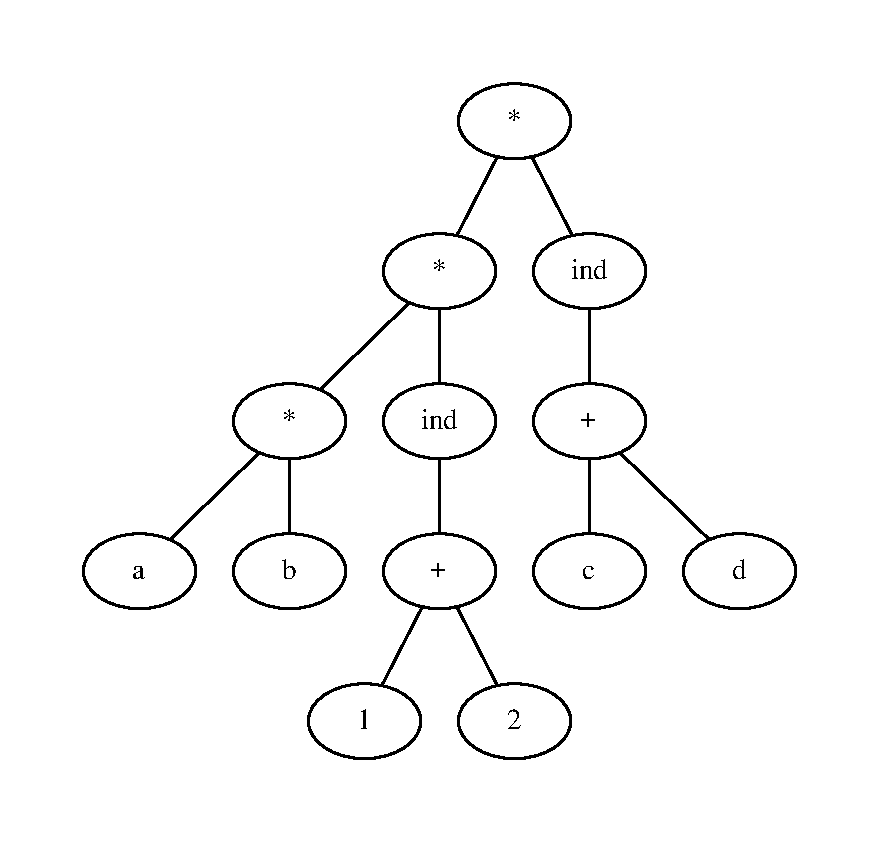
\includegraphics[scale=0.8]{expression_tree.pdf}
\caption{Input expression tree}
\label{fig:expression}
\end{figure}

\begin{figure}[!htb]
\centering
\hspace*{-1.5cm}
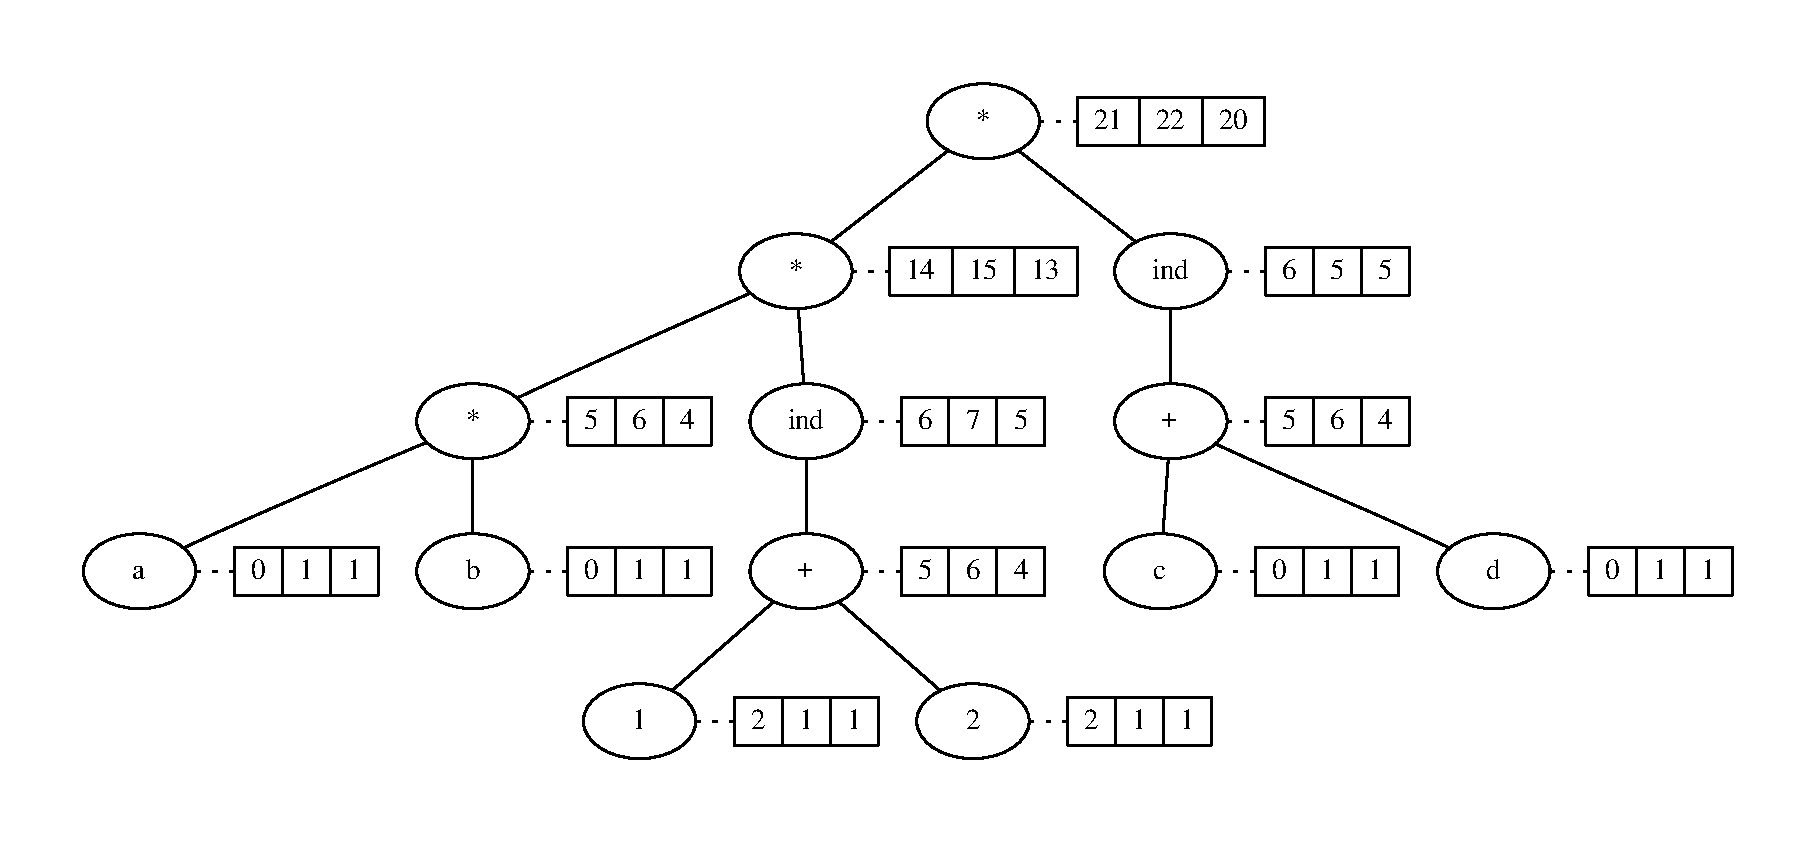
\includegraphics[scale=0.5]{phase1.pdf}
\caption{Output of phase 1 (Showing cost arrays only)}
\label{fig:expression}
\end{figure}

\textbf{\emph{cover(E,S)}} : Given an instruction and a node in an expression tree, \emph{cover(E,S)} returns True or False depending on whether the instruction(E) covers the node(S) or not. If the instruction(E) covers the node(S) then cover will place into two (initially empty) sets, \emph{regset} and \emph{memset}, the subtrees which need to be computed in registers and memory, respectively.\\\\

\textbf{\emph{Cost Array}} : This is an array of size $n + 1$ at each node.
\begin{itemize}
\item $C_j(S), j \neq 0$ : is the minimum cost of evaluating $S$ with a strong normal form program using $j$ registers.
\item $C_0(S)$ : cost of evaluating $S$ with strong normal form program in a memory location.\citep{sanyalcode}\\
\end{itemize}

\textbf{\emph{Optimal Instruction}} : From all the instructions which cover this node, optimal instruction gives the minimum cost. This is defined for each $C_j$.\\\\

\textbf{\emph{Optimal Permutation}} : The order in which the regset of the optimal instruction should be evaluated so that the cost will be optimum. This is defined for each $C_j$.\\\\


\subsection{Phase 2 : Determining the subtrees to be stored}
Phase 2 walks over the tree $T$, making use of the $C_j(S)$ arrays computed in Phase 1 to create a sequence of vertices $x_i, \dots, x_s$ of $T$. These vertices are the roots of those subtrees of $T$ which must be computed into memory; $x_s$ is the root of $T$.
These subtrees are so ordered that for all $i$, $x_i$ never dominates any $x_j$ for $j > i$. Thus if one subtree S requires some of its subtrees to be computed into memory, these subtrees will be evaluated before $S$ is evaluated. \emph{Phase 2} uses \emph{mark(T,n)}.

\textbf{\emph{mark(E,S)}} : Given a expression tree with costs (T) and number of registers(n), \emph{mark(T,n)} returns list of nodes in the given tree which need to be stored in memory for optimal cost.

\begin{figure}[!htb]
\centering
\hspace*{-1.5cm}
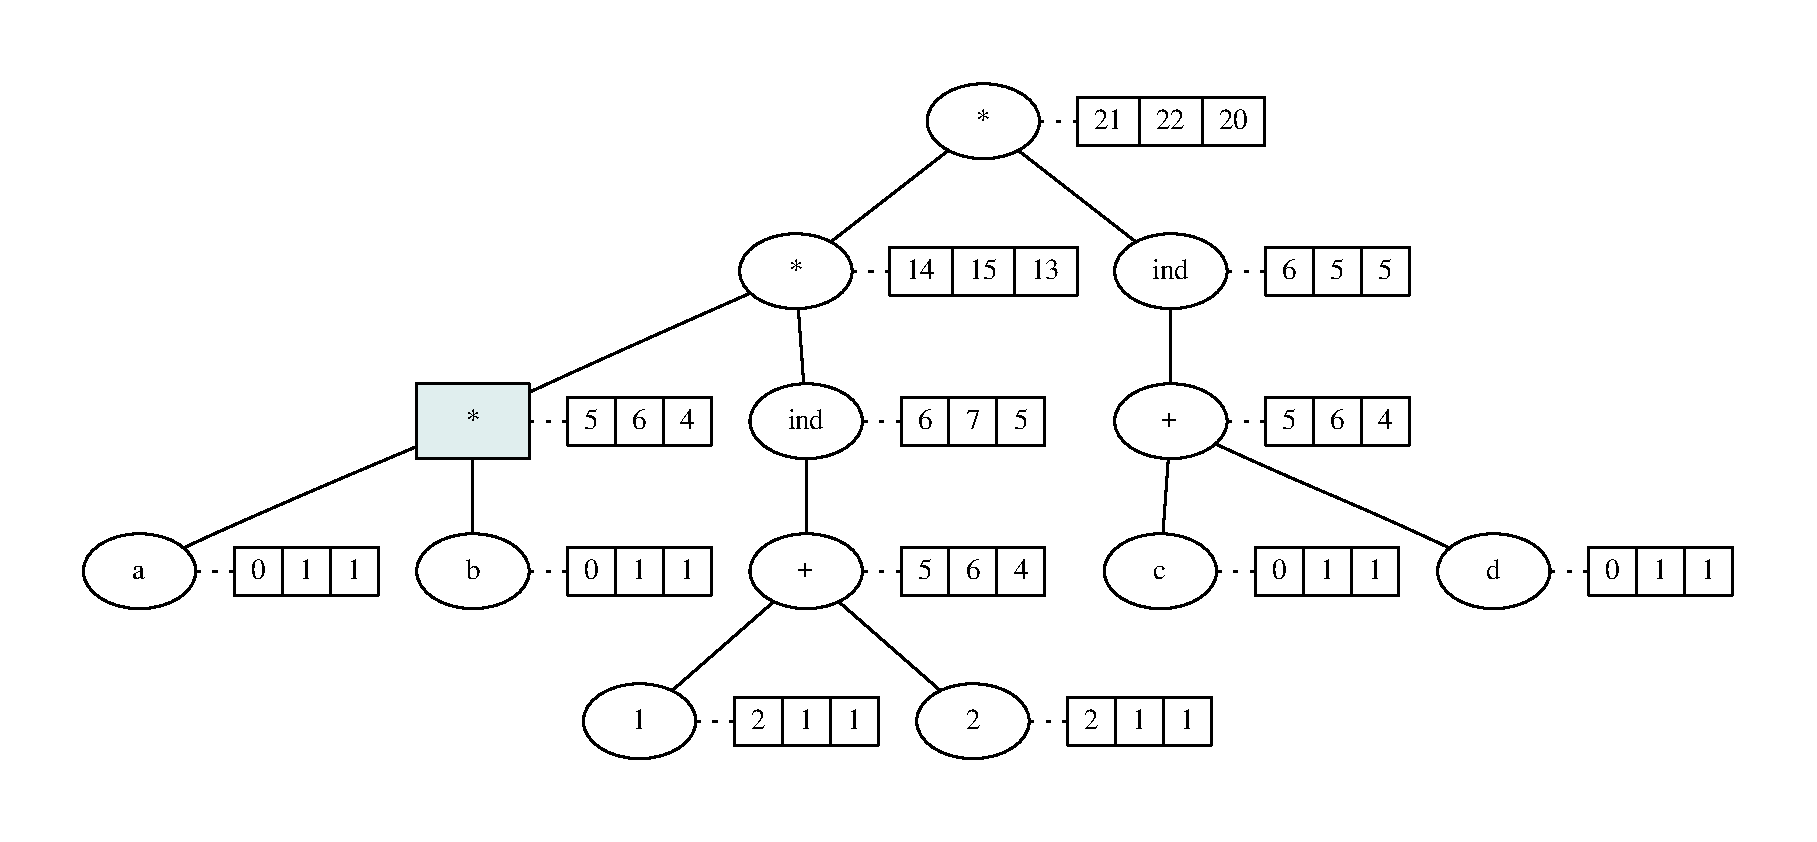
\includegraphics[scale=0.5]{phase2.pdf}
\caption{Phase 2 output}
\label{fig:expression}
\end{figure}


\subsection{Phase 3 : Code Generation}
This phase makes a series of walks over subtrees of T, generating code. These walks start at the vertices $x_i, \dots, x_s$ computed in Phase 2. After each walk, we generate a store into a distinct temporary memory location $m_i$, and rewrite node $x_i$, to make it behave like an input variable $m_i$ in later walks that might
encounter it. \emph{Phase 3} uses \emph{code(S,j)} to generate code.

\textbf{\emph{code(S,j)}} : Given a node(S) in expression tree which need to be stored in memory and number of registers(j), \emph{code(S,j)} returns sequence of instruction which results in optimal cost for give node(S).\\\\

Generated code:\\

\fbox{\parbox{0.36\linewidth}{
\texttt{r1 $\leftarrow$ b\\
r2 $\leftarrow$ a\\
r2 $\leftarrow$ (r2 * r1)\\
m1 $\leftarrow$ r2\\
r1 $\leftarrow$ 2\\
r2 $\leftarrow$ 1\\
r2 $\leftarrow$ (r2 + r1)\\
r2 $\leftarrow$ (ind r2)\\
r1 $\leftarrow$ m1\\
r1 $\leftarrow$ (r1 * r2)\\
r2 $\leftarrow$ c\\
r2 $\leftarrow$ (ind (r2 + d))\\
r1 $\leftarrow$ (r1 * r2)}
}}

\section{Implementation}

In this section we will describe how we implemented the Aho-Johnson algorithm in Haskell.
  
The final distributable after compilation is an executable called \texttt{Main}.

The usage of the program is:

\texttt{Main <number-of-registers> <instructions-file> <expression-tree-file> <output-file>}
  
\subsection{Definitions}

\begin{lstlisting}[language=Haskell]
type RegisterName = Int
type MemoryName = String
type Op = String
type Cost = Int

type RegSet = [Expr]
type MemSet = [Expr]

type Walk = [Int]

data Annotation = Annotation
    { costs :: [Cost]
    , instructions :: [Instruction]
    , permuts :: [[Int]]
    } deriving (Show, Read)

data Expr = Fork Op [Expr]
          | Register RegisterName
          | Constant Int
          | Memory MemoryName deriving (Show, Read, Eq)

data AnnotatedExpr = ForkAnnotated Op [AnnotatedExpr] Annotation
                   | RegisterAnnotated RegisterName Annotation
                   | ConstantAnnotated Int Annotation
                   | MemoryAnnotated MemoryName Annotation deriving (Show, Read)

data Instruction = RegisterAssign RegisterName Expr Cost
                 | Load RegisterName MemoryName Cost
                 | LoadConstant RegisterName Int Cost
                 | Store MemoryName RegisterName Cost
                 | NoInstruction deriving (Read, Eq)
\end{lstlisting}

\subsubsection{Sample instructions}

\setlength{\tabcolsep}{0.3cm}
\hspace*{-1.8cm}
\begin{tabular}{c|l}
 \textbf{Instruction} & \textbf{Haskell representation} \\ \hline
 $m \leftarrow r_1$ (Cost 4) & \texttt{Store "m" 1 4} \\
 $r_1 \leftarrow m$ (Cost 4) & \texttt{Load 1 "m" 4} \\
 $r_1 \leftarrow 2$ (Cost 5)& \texttt{LoadConstant 1 2 5} \\
 $r_1 \leftarrow r_1 + r_2$ (Cost 4) & \texttt{RegisterAssign 1 (Fork "+" [Register 1, Register 2]) 4} \\
 $r_1 \leftarrow ind (r_1 + m)$ (Cost 3)& \texttt{RegisterAssign 1 (Fork "ind" [Fork "+" [Register 1, Memory "m"]]) 3} 
\end{tabular}

\subsubsection{Sample expression}

\begin{lstlisting}[language=Haskell]
Fork "*" [Fork "*" [Fork "*" [Memory "a", Memory "b"], Fork "ind" [Fork "+" [Constant 1, Constant 2]]], Fork "ind" [Fork "+" [Memory "c", Memory "d"]]]
\end{lstlisting}

\subsection{Algorithm}

\begin{algorithm}[H]
 \texttt{instructions} $\leftarrow$ read the provided instructions file\;
 \texttt{expressionTree} $\leftarrow$ read the expression tree from provided file\;
 \texttt{n} $\leftarrow$ number of registers\;
 verify the number of registers\;
 verify instruction set\;
 verify expression tree\;
 generate PDF file for expressionTree using GraphViz\citep{GraphViz} tool (\texttt{dot} command)\;
 \texttt{initTree} $\leftarrow$ \texttt{initAnnotatedExprTree n expressionTree}\;
 \texttt{costTree} $\leftarrow$ \texttt{phase1 n instructions initTree}\;
 generate PDF file for costTree\;
 \texttt{markedNodes} $\leftarrow$ \texttt{phase2 n costTree}\;
 generate PDF file for costTree showing marked nodes\;
 \texttt{generatedCode} $\leftarrow$ \texttt{phase3 numberOfRegisters costTree marked}\;
 \caption{Main flow of the implementation}
\end{algorithm}

\subsection{Important functions}

\begin{lstlisting}[language=Haskell]
cover :: Instruction -> Expr -> (Bool, [Walk], [Walk])

initAnnotatedExprTree :: Int -> Expr -> AnnotatedExpr

--Call phase1AtNode recursively in preorder
phase1 :: Int -> [Instruction] -> AnnotatedExpr -> AnnotatedExpr

--Calculate costs at this node only, no recursion
phase1AtNode :: Int -> [Instruction] -> AnnotatedExpr -> AnnotatedExpr

phase2 :: Int -> AnnotatedExpr -> [Walk]
phase2 n tree = mark n n [] [] tree

--Recursive implementation of mark
mark :: Int -> Int -> Walk -> [Walk] -> AnnotatedExpr -> [Walk]

phase3 :: Int -> AnnotatedExpr -> [Walk] -> [Instruction]

--Called in phase3 for each marked node
code :: Walk -> Int -> AnnotatedExpr -> [RegisterName] -> [Instruction] -> (RegisterName, [Instruction], [RegisterName])
\end{lstlisting}

\section{Conclusion}
Implementing recursive algorithms in Haskell is really easy, and this algorithm is no exception. Tracking down bugs during development was really fast. As opposed to imperative languages, where due to side effects, bugs can occur anywhere (outside the function which actually has the bug).

\begin{itemize}
\item 
The time required by Phase 1 is $an$, where $a$ is a constant depending
\begin{enumerate}
\item linearly on the size of the instruction set
\item exponentially on the arity of the machine, and
\item linearly on the number of registers in the machine
\end{enumerate}
\item Time required by Phase 2 and 3 is proportional to $n$.
\end{itemize}


\bibliographystyle{plain}
\bibliography{references}
\end{document}
